\chapter{長い弦とブラックホール対応}

\lectureoverview{ブラックホールはエントロピーをもつので、微視的自由度をもたなければならない。我々はそれらの自由度について最も単純な弦理論的説明を構成する。まず長く励起された弦の状態を数え、次に弦結合定数を変化させて、弦とブラックホールの記述が出会うところを探る。最後の等号は、次の講義で完成させるべき問題として意図的に残しておく。}

\section{エントロピーは微視的担い手を要求する}

系が大きなエントロピーをもつということは、それが大量の微視的情報を隠しうるということである。熱い湯を張った浴槽は程度\(10^{30}\)のエントロピーをもちうる。この言明は、我々がそれを分子ごとに調べることを選ぶかどうかにかかわらず、膨大な数の微視的自由度が存在することをすでに告げている。熱力学はエネルギーと温度を測定することによってエントロピーを決定できるが、それを担う対象を特定するわけではない。

流体力学はこの区別を身近なものにする。それは原子に言及することなく、密度、速度、圧力、巨視的流れを記述する。熱力学を加えると、流体がエントロピーをもつことがわかる。エントロピーは、粗視化された方程式が示さない微視的構造を告げ知らせる。それは答えを与えるのではなく、新たな問いを招くのである。

ブラックホールは同じ難題をより鋭い形で提示する。ベッケンシュタインの提案は、ホーキングの計算によって完成され、地平線面積に比例するエントロピーを割り当てる。一般相対性理論は幾何とその熱力学を決定するが、微視的状態の目録を与えることはない。面積則を説明する配置をもつ、小さく多数の対象とは何か。弦理論には具体的な候補がある。ここで展開する議論は意図的に定性的である。それは数値定数や完全な状態数の形式的機構を抑えつつ、パラメータ依存性を正しく捉える。

\section{三つのスケールと一つの記法上の危険}

重力は特別な長さ、すなわちプランク長を与える。
\begin{equation}
\ell_p=\sqrt{\frac{G_N\hbar}{c^3}}.
\label{eq:l06-planck-si}
\end{equation}

\begin{classroomqa}
\audiencequestion{\(G_N\)、\(\hbar\)、\(c\)のどの組み合わせがプランク長を与えるか。\lecturetimestamp{00:06:08}}
\lecturerresponse{それは\(\sqrt{G_N\hbar/c^3}\)であり、およそ\(10^{-33}\)センチメートルである。我々は直ちに\(\hbar=c=1\)と置くので、関係はずっと簡単になる。}
\end{classroomqa}

自然単位では、
\begin{equation}
\hbar=c=1,
\qquad
G_N=\ell_p^2.
\label{eq:l06-planck-area}
\end{equation}
したがってニュートン定数は面積の次元をもつ。これが、面積を\(G_N\)で割ったものが無次元であり、エントロピーになりうる理由である。

弦理論には第二の長さ\(\ell_s\)がある。弦を熱するか、あるいは高度に励起された状態に置くと、それは多くのスケールで揺れる。この初等的な描像における特徴的な最短スケールは弦の長さである。\(\ell_s\)を、弦振動の一つの素励起単位に付随する大きさとみなしてよい。

第三の量は無次元の弦結合定数\(g_s\)である。それは分裂と結合を支配する。弦は二本の弦にくびれて分かれることができ、あるいは励起された弦は閉弦量子を放出できる。

\begin{classroomqa}
\audiencequestion{弦結合定数の物理的意味は何か。\lecturetimestamp{00:09:20}}
\lecturerresponse{それは、弦が自己交差するときの分裂のような、弦の相互作用の確率を支配する。より正確には、\(g_s\)は相互作用振幅であり、対応する確率や率は\(g_s^2\)の次数から始まる。}
\end{classroomqa}

放出される質量ゼロの閉弦励起はグラビトンでありうる。その点で\(g_s\)は電荷に類似した役割を果たす。すなわち、それは相互作用の頂点に付随する因子である。\editorialnote{この講義では\(g_s\)を確率と呼んだり振幅と呼んだりしている。摂動的にはそれは振幅レベルの結合定数であり、確率と率はその二乗を含む。}

\section{重力はなぜ\texorpdfstring{\(g_s^2\)}{結合定数の二乗}を知っているのか}

まず電磁気学の交換描像を考える。一つの荷電物体が因子\(e\)を伴って光子を放出し、第二の物体がもう一つの因子\(e\)を伴ってそれを吸収する。したがって交換振幅は\(e^2\)を含む。この描像は文字通りの古典的発射物の話ではないが、結合定数がどのように入るかを正しく示している。

\begin{figure}[htbp]
\centering
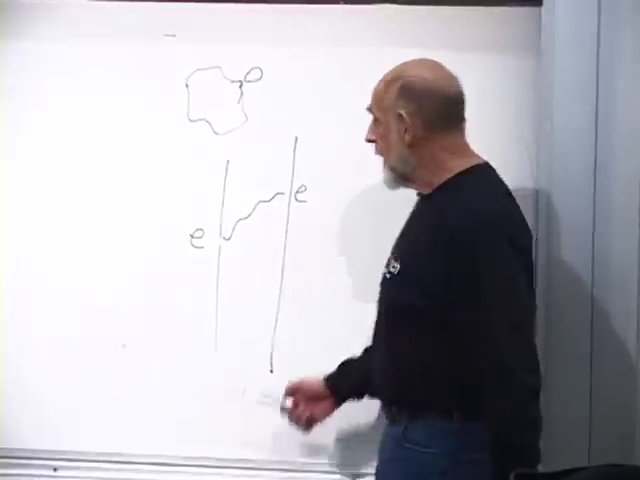
\includegraphics[width=0.72\textwidth]{lecture_06_figure_03.png}
\caption{黒板に描かれた完成した交換のスケッチ。結合定数が放出の際に、そして再び吸収の際に付随する。}
\lectureframe{00:11:30.000}
\end{figure}

弦理論版では光子をグラビトンに、電荷を\(g_s\)に置き換える。一つの因子が放出に伴い、もう一つが吸収に伴うので、重力の強さは\(g_s^2\)でスケールする。

長距離では、同じ相互作用がニュートンの力の法則を再現しなければならない。
\begin{equation}
F_{\mathrm{grav}}\sim G_N\frac{M_1M_2}{r^2}.
\end{equation}
質量と逆二乗依存性は源と伝播を記述する。ここで必要な点は、それらに掛かる結合定数である。

\begin{figure}[htbp]
\centering
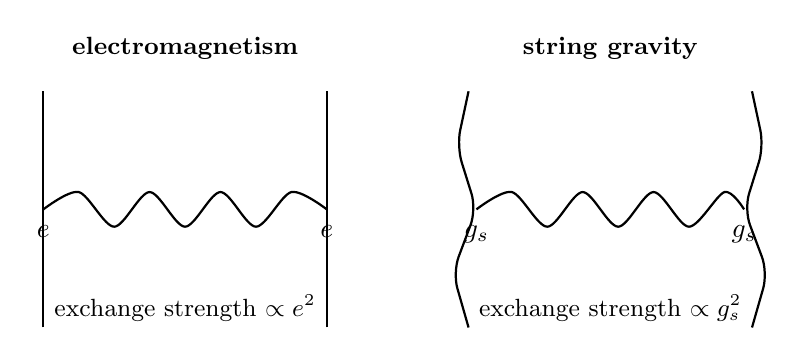
\begin{tikzpicture}[x=1cm,y=1cm]
  \node[font=\small\bfseries] at (1.8,3.55) {electromagnetism};
  \draw[line width=0.8pt] (0,0) -- (0,3);
  \draw[line width=0.8pt] (3.6,0) -- (3.6,3);
  \draw[line width=0.8pt] plot[smooth] coordinates {(0,1.5) (0.45,1.72) (0.9,1.28) (1.35,1.72) (1.8,1.28) (2.25,1.72) (2.7,1.28) (3.15,1.72) (3.6,1.5)};
  \node[below] at (0,1.42) {\(e\)};
  \node[below] at (3.6,1.42) {\(e\)};
  \node[font=\small] at (1.8,0.25) {exchange strength \(\propto e^2\)};
  \node[font=\small\bfseries] at (7.2,3.55) {string gravity};
  \draw[line width=0.8pt,rounded corners=6pt] (5.4,0) -- (5.2,0.7) -- (5.5,1.5) -- (5.25,2.3) -- (5.4,3);
  \draw[line width=0.8pt,rounded corners=6pt] (9,0) -- (9.2,0.7) -- (8.9,1.5) -- (9.15,2.3) -- (9,3);
  \draw[line width=0.8pt] plot[smooth] coordinates {(5.5,1.5) (5.95,1.72) (6.4,1.28) (6.85,1.72) (7.3,1.28) (7.75,1.72) (8.2,1.28) (8.65,1.72) (8.9,1.5)};
  \node[below] at (5.5,1.42) {\(g_s\)};
  \node[below] at (8.9,1.42) {\(g_s\)};
  \node[font=\small] at (7.2,0.25) {exchange strength \(\propto g_s^2\)};
\end{tikzpicture}
\caption{結合の数え方の類推。交換される量子の各端が1つの相互作用因子を与える。}
\end{figure}

この観察はニュートン定数をほとんど決定する。結合定数\(g_s\)は無次元であり、一方、四次元では\(G_N\)は長さの二乗の次元をもつ。利用可能な微視的長さは\(\ell_s\)であるから、
\begin{equation}
G_N\sim g_s^2\ell_s^2.
\label{eq:l06-newton-string}
\end{equation}
これと式~\eqref{eq:l06-planck-area}を組み合わせると、
\begin{equation}
\ell_p\sim g_s\ell_s.
\label{eq:l06-planck-string}
\end{equation}

\begin{figure}[htbp]
\centering
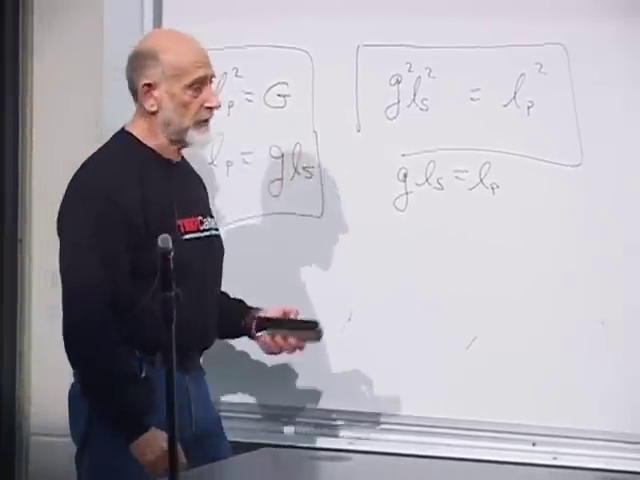
\includegraphics[width=0.72\textwidth]{lecture_06_figure_04.png}
\caption{黒板に残された基本関係式：\(\ell_p^2=G_N\)および\(\ell_p\sim g_s\ell_s\)。}
\lectureframe{00:15:45.000}
\end{figure}

式~\eqref{eq:l06-newton-string}はこの講義全体で用いられる簡略化された関係式である。\editorialnote{コンパクト化された弦理論では、有効4次元ニュートン定数はコンパクト化体積と1の程度の規約にも依存する。講義ではそれらのデータを抑え、対応関係のスケーリングを際立たせている。}

\begin{classroomqa}
\audiencequestion{\(g_s\)は1より大きいか小さいか、そしてどちらの長さがより大きいか。\lecturetimestamp{00:16:00}}
\lecturerresponse{我々は弱結合\(g_s<1\)で考える。すると\(\ell_p\sim g_s\ell_s\)は弦の長さがプランク長さより大きいことを意味する。強結合は別の記述を必要とし、ここでは不要である。}
\end{classroomqa}

\section{ブラックホールの数え上げ}

ボルツマン定数と数値因子を抑えると、ベッケンシュタイン--ホーキングエントロピーは
\begin{equation}
S_{\mathrm{BH}}=\frac{A}{4G_N}sim\frac{A}{G_N}sim\frac{A}{\ell_p^2}.
\label{eq:l06-bh-area}
\end{equation}
因子\(1/4\)は半古典的公式において厳密であるが、このスケーリングの議論では役割を果たさない。

\begin{classroomqa}
\audiencequestion{添字``BH''はブラックホールを意味するのか、それともベッケンシュタイン--ホーキングを意味するのか。\lecturetimestamp{00:16:51}}
\lecturerresponse{我々の目的には、両方を思い起こさせるものであればよい。重要なのは、エントロピーがプランク面積で測った事象の地平面の面積であるという点である。}
\end{classroomqa}

4次元シュヴァルツシルトブラックホールに対して、
\begin{equation}
R_s=2G_NM,
\qquad
A=4\pi R_s^2.
\end{equation}
講義でそうするように\(2\)と\(4\pi\)を落とすと、
\begin{align}
S_{\mathrm{BH}}
&\sim \frac{R_s^2}{G_N}
\sim \frac{(G_NM)^2}{G_N} \\
&\sim M^2G_N
\sim M^2\ell_p^2.
\label{eq:l06-bh-mass}
\end{align}
これが我々が弦の数え上げと比較する形である。

\section{長い弦のランダムウォークとしての描像}

小さな弦から始めて、それにエネルギーを注ぎ込む。一般の高度に励起された弦は整ったループのままではいない。それは、ひどく絡まったリールから出た釣り糸のように、長く絡み合った対象となる。巨視的に見て同じに見える配位が膨大に存在するため、この絡まりはエントロピーをもつ。

それらを数えるために、空間をリンクの長さが\(\ell_s\)である格子で置き換える。サイトは頂点、リンクは線分、基本正方形はプラケットである。弦はリンクの連結した列で表される。この模型は意図的に粗いものであるが、その指数的な状態数は望ましいスケーリングを捉えている。

\begin{figure}[htbp]
\centering
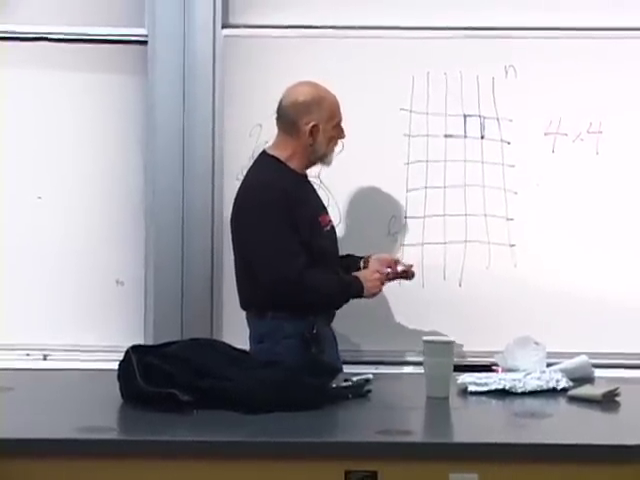
\includegraphics[width=0.72\textwidth]{lecture_06_figure_05.png}
\caption{2次元格子模型。青い線分は弦の1ステップを示し、各サイトで4つの可能な継続が数えられる。}
\lectureframe{00:23:50.000}
\end{figure}

\begin{classroomqa}
\audiencequestion{おもちゃのウォークの各ステップで何通りの選択肢があるか。\lecturetimestamp{00:22:43}}
\lecturerresponse{正方形格子上では4通りである。即座の後戻りが許されるからである。3次元では6通りになるであろう。別の格子ではその通常の数は変わるが、ウォークの数がリンクの数に対して指数的に増大するという事実は変わらない。}
\end{classroomqa}

弦が\(n\)個のリンクをもつなら、2次元のおもちゃの数え上げは
\begin{equation}
\Omega_n\sim4^n.
\label{eq:l06-walk-count}
\end{equation}
例外的な直線ウォークが1つあるが、それは\(4^n\)個のうちの1つの状態にすぎない。典型的なウォークは繰り返し折り畳まれ、絡まった球を占める。大きな\(n\)に対して、ランダムに生成されたほとんどすべての配位は定性的に他のすべてと同じに見える。

エントロピーは巨視的に区別できない配位の数の対数である：
\begin{equation}
S_{\mathrm{st}}=\log\Omega_n\sim n\log4\sim n.
\label{eq:l06-string-entropy-n}
\end{equation}

\begin{classroomqa}
\audiencequestion{なぜエントロピーは\(4^n\)ではなく\(n\)に比例するようになるのか。\lecturetimestamp{00:25:39}}
\lecturerresponse{エントロピーは状態数の対数である。したがって\(\log(4^n)=n\log4\)であり、因子\(\log4\)は1の程度の定数であり、我々はそれを抑える。}
\end{classroomqa}

\(L\)が弦を一端から他端までたどって得られる輪郭長であるなら、
\begin{equation}
n=\frac{L}{\ell_s},
\qquad
S_{\mathrm{st}}\sim\frac{L}{\ell_s}.
\label{eq:l06-string-entropy-length}
\end{equation}
ここで\(L\)は絡まった球の直径ではない。それは弦に沿って測ったはるかに長い距離である。

次に輪郭長を質量と交換する。\(c=\hbar=1\)のもとで、質量は逆長さの次元をもつ。したがって弦の大きさの1つのリンクは程度
\begin{equation}
m_{\mathrm{link}}\sim\frac{1}{\ell_s}.
\label{eq:l06-link-mass}
\end{equation}
の質量を担う

\begin{classroomqa}
\audiencequestion{なぜ1つのリンクの質量は\(1/\ell_s\)としてスケールしなければならないのか。\lecturetimestamp{00:29:20}}
\lecturerresponse{これらの単位では質量は逆長さであり、\(\ell_s\)が唯一利用可能な長さである。同等に、程度\(1/\ell_s^2\)の弦の張力にリンク長\(\ell_s\)を掛けると同じ結果を与える。}
\end{classroomqa}

すると完全な弦は
\begin{equation}
M\sim n m_{\mathrm{link}}
\sim\frac{n}{\ell_s}
\sim\frac{L}{\ell_s^2},
\qquad
L\sim M\ell_s^2.
\label{eq:l06-string-mass}
\end{equation}
となる。式~\eqref{eq:l06-string-entropy-length}に代入すると
\begin{equation}
S_{\mathrm{st}}\sim M\ell_s.
\label{eq:l06-string-entropy-mass}
\end{equation}
が得られる。格子ウォークは世界面の拘束条件と数値係数を無視しているが、高度に励起された弦スペクトルの指数的成長がこの同じ主要なスケーリングを与える。\editorialnote{このランダムウォーク構成は弦状態の高準位密度のための記憶術であり、基本弦の文字通りの離散化ではない。}

\section{議論の出発点となる不一致}

二つの答えは今や
\begin{equation}
S_{\mathrm{BH}}\sim M^2\ell_p^2,
\qquad
S_{\mathrm{st}}\sim M\ell_s.
\label{eq:l06-two-entropies}
\end{equation}
である。それらは互いに似ているが、固定された質量と任意の結合定数において等しくはない。ブラックホールの表式は\(M\)について二次であり、弦の表式は線形である。高温の弦が単にブラックホールであると宣言することはできない。二つの領域がどのように接続するかを説明しない限り。

\begin{figure}[htbp]
\centering
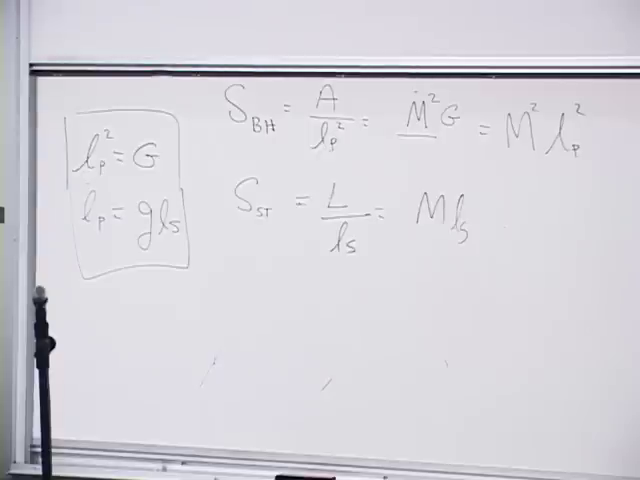
\includegraphics[width=0.78\textwidth]{lecture_06_figure_06.png}
\caption{妨げのないボード比較：上にブラックホールエントロピー、下に長い弦のエントロピー、左にプランク--弦関係を保持。}
\lectureframe{00:33:20.000}
\end{figure}

ここで講義は中断した。このサスペンスは有用である。不一致はアイデアの失敗ではなく、重力の強さを変えながら同じ状態を比較しなければならないという手がかりである。

\section{結合定数のつまみを回す}

\(\ell_s\)を固定し、\(g_s\)が変化しうると想像する。\(g_s=0\)では、弦は分裂も結合もせず、\(G_N\sim g_s^2\ell_s^2\)であるため重力は消える。十分にエネルギーの高い状態は、そのとき長く弱く相互作用する弦である。

\(g_s\)をゆっくり増加させる。弦の相互作用が可能になり、そして現在の議論にとってより重要なことに、重力が強くなる。

\begin{classroomqa}
\audiencequestion{\(g_s\)が増加するとき、最初の効果は単に弦がより短い弦に分裂することだろうか。\lecturetimestamp{00:36:29}}
\lecturerresponse{分裂と結合が可能になるが、\(\ell_s\)を固定し、高エントロピー状態を追跡する。中心的な効果は\(G_N\)が成長することであり、それゆえ長い弦の自己重力がもつれた球を内側に引き寄せる。}
\end{classroomqa}

物体は収縮し、より高密度になる。その重力ポテンシャルエネルギーは負であるため、収縮はその全エネルギーを低下させ、したがってその質量を低下させる。

\begin{classroomqa}
\audiencequestion{自己重力が弦を引き寄せるにつれて、エネルギーは増加するか減少するか。\lecturetimestamp{00:37:48}}
\lecturerresponse{減少する。結合エネルギーがより負になる。同じ状態を追跡し続けているにもかかわらず、経路上の質量は固定されている必要はない。}
\end{classroomqa}

最終的に物体の大きさはそのシュヴァルツシルト半径に匹敵する。その点を超えると、ブラックホールの記述が自然なものとなる。より大きな初期励起は、より小さな結合定数でこの条件に達する。なぜなら、より重い物体は地平線を形成するためにより少ない重力の強さを必要とするからである。

\begin{figure}[htbp]
\centering
\resizebox{0.95\linewidth}{!}{%
\begin{tikzpicture}[x=1cm,y=1cm,>=Latex]
  \draw[->,line width=0.9pt] (0,0) -- (11,0) node[right] {increasing \(g_s\)};
  \node[draw,rounded corners,align=center,minimum width=2.6cm,minimum height=1.15cm] at (1.8,1.5) {long excited string\\weak self-gravity};
  \node[draw,rounded corners,align=center,minimum width=2.6cm,minimum height=1.15cm] at (5.5,1.5) {correspondence point\\\(R_s\sim\ell_s\)};
  \node[draw,circle,align=center,minimum size=1.8cm] at (9.3,1.5) {black\\hole};
  \draw[->,line width=0.8pt] (3.15,1.5) -- (4.1,1.5) node[midway,above,font=\small] {contracts};
  \draw[->,line width=0.8pt] (6.9,1.5) -- (8.25,1.5);
  \node[font=\small,align=center] at (5.5,-0.65) {same family of states followed slowly;\\binding energy and mass may change};
\end{tikzpicture}
}
\caption{固定された\(\ell_s\)における対応の経路。矢印を逆にたどると、ブラックホール状態が長い弦の状態に戻る。}
\end{figure}

\begin{classroomqa}
\audiencequestion{\(g_s\)がゼロと1の間にあると想像すべきだろうか。\lecturetimestamp{00:40:18}}
\lecturerresponse{はい。議論は弱結合領域にとどまる。\(g_s\)が非常に小さければ、ブラックホールになる前に状態は相応に重くなければならない。制御が不十分な\(g_s>1\)領域に入る必要はない。}
\end{classroomqa}

この思考実験において、ゆっくりした変化は可逆である。

\begin{classroomqa}
\audiencequestion{重力がもはやブラックホールをまとめておけないところまで結合定数を再び下げると、それは何になるか。\lecturetimestamp{00:41:37}}
\lecturerresponse{長い弦である。重力が消えるとき、この構成のすべては弦状態で記述されなければならない。つまみを一方に回すと弦がブラックホールに写像され、逆に回すとブラックホールが弦に写像される。}
\end{classroomqa}

固定された全エネルギーと固定された体積の下で、支配的な高エントロピー配置は、膨大な数の短い弦ではなく、本質的に一つの長い弦である。この主張はここでは導出されない。それはハゲドルン領域近傍における弦の統計力学の結果であり、再び取り上げられるであろう。

\section{外部の観測者が見るもの}

物体がブラックホールとして記述されるとき、弦はどこにあるのか。外部の記述では、それは突然消えるのではない。シュヴァルツシルト時間は見かけの横断を任意に遅い時間へと送るので、弦的な自由度は地平線上またはその近くに蓄積するものとして表される。

\begin{figure}[htbp]
\centering
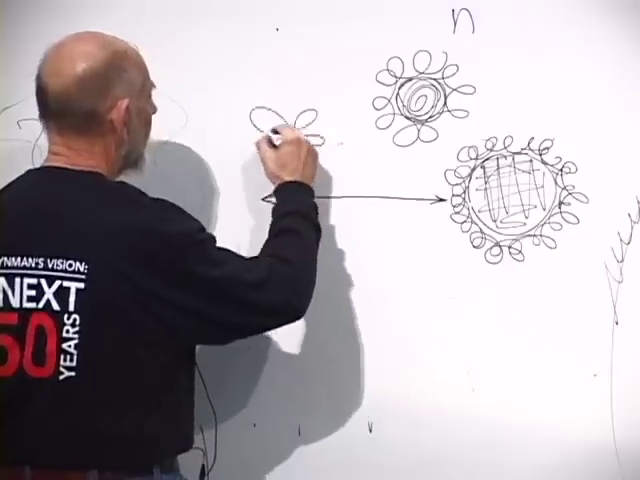
\includegraphics[width=0.72\textwidth]{lecture_06_figure_07.png}
\caption{巨視的な地平線——そこでは弦スケールの構造が薄い綿毛である——と、半径がループスケールに近づくより小さな地平線とのボード比較。}
\lectureframe{00:45:30.000}
\end{figure}

\(R_s\gg\ell_s\)では、ブラックホールは巨視的であり、弦スケールの構造は事象の地平面半径に対して薄い層にすぎない。半径が\(\ell_s\)に向かって減少するにつれて、滑らかなブラックホールと伸長した弦との区別は意味を失う。これは外部からの、引き伸ばされた地平面による記述であり、落下する物質が正則な地平面を決して横切らないという座標に依存しない主張と混同してはならない。\editorialnote{この講義では、ブラックホール相補性でよく知られた外部記述を用いる。``地平面上''という語句は、外部記述によって分解される自由度を指し、それらの共変的な位置を別途導出するものではない。}

クロスオーバーは次式のときに起こる。
\begin{equation}
R_s\sim\ell_s.
\label{eq:l06-correspondence-radius}
\end{equation}
弦スケール以下では、シュヴァルツシルト幾何はそれを支えるはずの構造を分解できない。ループは本来の地平面から揺らぎ離れ、その状態はむしろ弦と呼ぶのが適切である。

\section{対応点}

式~\eqref{eq:l06-correspondence-radius}において\(R_s\sim G_NM\)を用いる。
\begin{equation}
G_NM\sim\ell_s.
\end{equation}
次に\(G_N\sim g_s^2\ell_s^2\)を代入する。
\begin{equation}
M g_s^2\ell_s^2\sim\ell_s,
\qquad
M g_s^2\ell_s\sim1.
\label{eq:l06-correspondence-condition}
\end{equation}

\begin{figure}[htbp]
\centering
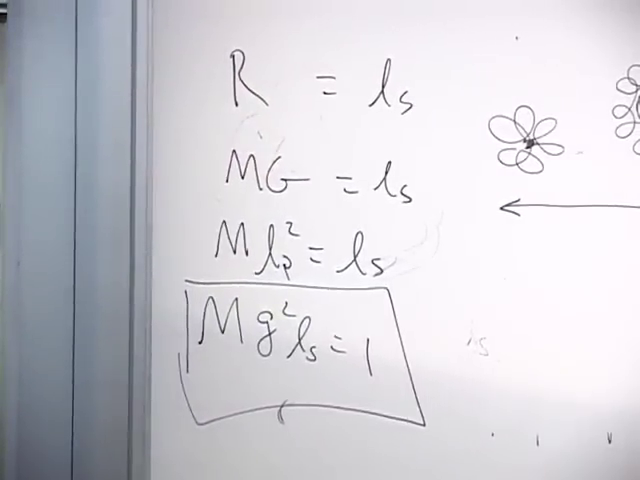
\includegraphics[width=0.72\textwidth]{lecture_06_figure_08.png}
\caption{黒板での完全な遷移の代数：\(R_s\sim\ell_s\)は枠で囲まれた無次元条件\(Mg_s^2\ell_s\sim1\)に至る。}
\lectureframe{00:49:50.000}
\end{figure}

聴衆の一人が、この条件が何を準備しているかに気づいた。対応点では、
\begin{align}
S_{\mathrm{BH}}
&\sim M^2\ell_p^2
\sim M^2g_s^2\ell_s^2 \\
&=(M\ell_s)(Mg_s^2\ell_s)
\sim M\ell_s
\sim S_{\mathrm{st}}.
\label{eq:l06-entropy-preview}
\end{align}

\begin{classroomqa}
\audiencequestion{これらの式はすでにブラックホールと弦のエントロピーが等しくなることを含意しているのか。\lecturetimestamp{00:50:18}}
\lecturerresponse{はい。まさにそこへ計算が向かっている。材料は黒板に置かれたが、講義は対応の論理を注意深く見直せるよう、それらの完全な組み立てを延期する。}
\end{classroomqa}

式~\eqref{eq:l06-entropy-preview}は、このやり取りに暗黙に含まれる一行の代数的予告である。それはスケーリングを確立するものであり、厳密な係数\(1/4\)ではない。厳密な微視的対応には、より制御されたブラックホールとより詳細な弦の構成が必要である。\editorialnote{講義は式~\eqref{eq:l06-entropy-preview}を完成した導出として提示する手前で止まっている。ここに書き出したのは、聴衆が明示的にこの等式を指摘し、必要な関係がすべてすでに現れているからである。}

\section{なぜエントロピーを持ち越せるのか}

論理的な材料がもう一つ残っている。磁場や\(g_s\)のような制御パラメータを、系が孤立し、その発展が可逆である間に十分ゆっくり変化させるとする。エネルギー、大きさ、束縛は変化しうるが、エントロピーは保存される。
\begin{equation}
\Delta S=0.
\label{eq:l06-adiabatic-entropy}
\end{equation}
講義はこれを情報の保存と結びつける。エントロピーは粗視化された記述によって隠された情報を測る。ハミルトニアンのゆっくりした可逆変化は、その情報を消すことなく状態を並べ替える。

\begin{classroomqa}
\audiencequestion{エントロピーが一定であるには、経路が相転移を避ける必要があるのか。\lecturetimestamp{00:54:01}}
\lecturerresponse{はい、状態を連続的に追跡できなければならない。有限系には無限体積の場合のような厳密に非解析的な熱力学的相転移はなく、変化が十分ゆっくりであれば、対応は滑らかなクロスオーバーとして扱える。}
\end{classroomqa}

ここで断熱とは、より強い準静的・可逆の意味で用いられている。断熱的だが不可逆な過程はエントロピーを生みうる。ゆっくりであることと状態を追跡できることが本質的である。\editorialnote{熱力学的な主張\(\Delta S=0\)には可逆な断熱経路が必要である。量子力学的には、対応する考え方は、制御されない準位遷移なしにパラメータが変化するにつれて同じ状態の集合を追跡することである。}

\begin{classroomqa}
\audiencequestion{同じ全質量を持つ複数の短い弦よりも、一つの長い弦の方がなぜエントロピーが大きいのか。\lecturetimestamp{00:54:44}}
\lecturerresponse{直感に反するが、高エネルギー状態の明示的な数え上げは、固定体積において長い弦の成分を有利にする。証明は後回しにする。現在の議論には、ブラックホールが非常に多くの短い弦の希薄な気体ではなく、最大エントロピーの弦のセクターに対応することだけが必要である。}
\end{classroomqa}

したがって操作的な戦略は次のとおりである。
\begin{enumerate}
\item 結合\(g_{s,0}\)において質量\(M_0\)のブラックホールから始める。
\item 同じ高エントロピー状態の族を追跡しながら\(g_s\)をゆっくり下げる。
\item ブラックホール記述が長い弦の記述になる\(R_s\sim\ell_s\)で止める。
\item \(S_{\mathrm{st}}\sim M\ell_s\)を用いて弦の状態を数える。
\item そのエントロピーを可逆経路に沿って元のブラックホールへ持ち戻す。
\end{enumerate}

\begin{figure}[htbp]
\centering
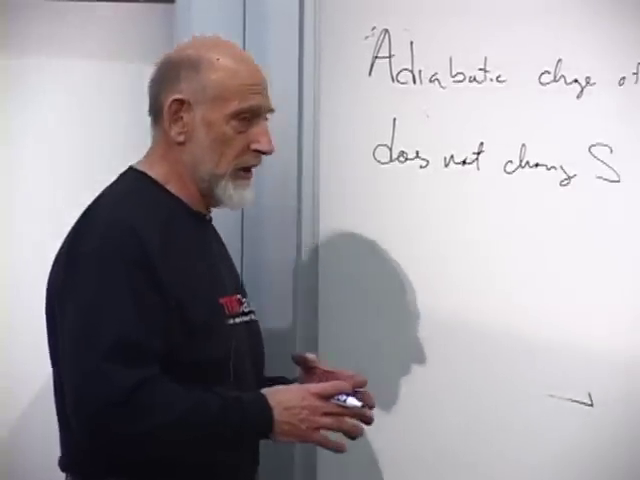
\includegraphics[width=0.72\textwidth]{lecture_06_figure_09.png}
\caption{戦略を述べる間、黒板に保たれる原理：\(g_s\)の断熱変化は\(S\)を変えない。}
\lectureframe{00:56:40.000}
\end{figure}

弦理論は、電荷をもつ回転する超対称な準極限および高次元ブラックホールに対して、はるかに精密なエントロピー数え上げを与えてきた。ここでの中性シュヴァルツシルトの議論は粗い対応関係の議論である。すなわち、状態密度のパラメトリックな振る舞いと物理的なクロスオーバーを同定するものであって、厳密に保護された縮退を与えるものではない。\editorialnote{厳密な一致が最も強いのは、結合定数が変化しても状態数が保護される特別なブラックホールに対してである。本講義では意図的に最も単純な桁程度の版を与えている。}

\begin{classroomqa}
\audiencequestion{重力を切ったとき、状態はちょうど1本ではなく2本の弦になりうるだろうか。\lecturetimestamp{00:58:25}}
\lecturerresponse{少数の長い弦に対しては有限の確率があり、1本ではなく2本を使っても主要なエントロピーのスケーリングは変わらない。議論を変えるのは、短い弦の巨大な気体への断片化である。高エネルギーでの統計的な数え上げはその結果を支持しない。}
\end{classroomqa}

ブラックホールはある領域に詰め込むことのできる最大のエントロピーであり、長い弦は重力を取り除いたときの対応する高エントロピー状態である。これら二つの記述は今や結びつけられているが、まだ精密計算へと展開されてはいない。次の段階は、代数を注意深く繰り返し、この対応がどこまで信頼できるかを問うことである。
